\documentclass{../../../../style/mkimain}

\series{4}
\month{květen}
\year{2023}

\begin{document}
%<*header>
\section*{IV.A Header4-A}
%</header>
Hned na začátek zapátrejme v paměti, a vzpomeňme si na seriál II.K.
V tomto seriálu jste se dozvěděli o \emph{Planckově vyzařovacím zákonu}.
Víte tedy, že každé těleso vyzařuje na všech vlnových délkách, avšak na jedné nejvíce.
A převážně tuto vlnovou délku vidíme.
Podle \emph{Wienova~posunovacího~zákona} je tato vlnová délka nepřímo úměrná teplotě tělesa.
To znamená, že čím vyšší teplota hvězdy je, tím více se maximání vlnová délka posouvá k modré části spektra.
Modré hvězdy jsou tedy teplejší než hvězdy červené.
%spektrum cerneho telesa

Při pohledu na hvězdnou oblohu si lze velmi snadno všimnout toho, že hvězdy jsou různě jasné.\footnote{Pro další čtení; je potřeba vnímat dvě odlišné veličiny: jasnost a zářivost/svítivost.}
Jak jasně hvězdu vidíme závisí na veličině, kterou nazýváme \emph{hustota zářivého toku}\footnote{V češtině se poměrně zmatečně může nazývat (bolometrická) jasnost.} a na vzdálenosti.
Prozatím vzdálenost odložíme, a budeme počítat s tím, že pozorujeme hvězdy ve stejné vzdálenosti.

Hustota zářivého toku (dále jen HZT) je veličina popisující tok záření, které projde $\qty{1}{\m\squared}$ za $\qty{1}{\s}$.
HZT dává do vztahu společne s teplotou tělesa \emph{Stefan-Boltzmannův zákon}.\footnote{V češtině by se správně mělo psát: Stefan\underline{ův}-Boltzmannův zákon – to nám však přijde opravdu uširvoucí.}
Ten říka, že HZT je přímo úměrná čtvrté mocnině teploty tělesa.
Proto, čím teplejší hvězda je, tím více energie vyzařuje – je jasnější.

Jako míru jasnosti používáme hvězdnou velkost, neboli \emph{magnitudu}.
Tato míra odpovídá historickému dělení hvězd do šesti skupin, kde 0 byla nejjasnější a 5 nejméně jasná.
Dnes však magnitudu používáme pro všechny objekty na obloze, proto může jít i do záporu.
Například, nejjasnější objekt na obloze – Slunce – má magnitudu $-26,6$.
Chceme-li však porovnávat magnitudu nezávisle na vzdálenosti objektu, používáme tzv. \emph{absolutní magnitudu}.
Jedná se magnitudu, jakou by mělo pozorované těleso kdybychom ho pozorovali ze vzdálenosti $\qty{10}{\parsec}$ od nás.

Různě veliké hvězdy mohou být stejně jasné (mít stejnou HZT), avšak budou různě zářivé.
Proto zavádíme další veličinu, která nám popisuje, jak hvězdu vidíme, a to \emph{zářivý výkon} (mohli bychom říct zářivost či svítivost).
Jak je ale možné, že dvě stejně jasné hvezdy uvidíme jinak zářivé?
Odpověd spočívá v odlišných rozměrech.
Hvězdy vyzařují energii svým povrchem.
Je-li jedna hvězda o stejné jasnosti vetší než druhá, tedy má větší povrch, bude zářit více.
Zkrátka, má vetší plochu, ze které září.
Není tedy težké domyslet, že zářivý výkon vypočítáme tak, že HZT vynásobíme povrchem hvězdy.

Jak jsme již na samém začátku avizovali, hvězdy mají různé barvy.
Neboli, světlo, které k nám od nich příchází, má různe spektrum.
Na základě toho byly vytvořeny tzv. \emph{spektrální třídy}.
Původně byly hvězdy rozděleny do sedmi skupin\footnote{Existuje mnoho vtipných pořekadel na zapamatování si všech tříd. Doporučujeme vám si je najít.}, kde každá skupina má deset podskupin.
S rozvojem techniky rozsah nestačil, a tak se třídy postupně rozrostly do dnešních třinácti.
Často se ale uvádí pouze sedm základních, jelikož další skupiny jsou zastoupeny jen zřídka.

Na začátku 20. století nezávisle na sobě dva astronomové zkonstruovali diagram, na kterém zaznamenávali absolutní magnitudu na svislou osu a spektrální třídu na vodorovnou osu.
Tento diagram se po nich nazývá \emph{Hertzsprung-Russelův diagram}.
Od svého vzniku však diagram prošel malými změnami.
Dnes již víme (a vy od minulého seriálu také!), že spektrální třída závisí na teplotě.
Proto se spíše častěji setkáte s diagramem, kde na vodorovné ose bude teplota.
Také víme, že absolutní magnituda závisí pouze na zářivém výkonu, proto je dnes na jedné svislé ose stupnice zářivého výkonu, a na druhé absolutní magnituda.
Co se však nezměnilo jest, že teplota se historicky zaznamenávala tak, že roste zprava doleva.

Při zanášení dat do diagramu si astronomové všimli, že diagram není vyplněn rovnoměrně, ale vzniklo v něm několik výrazně zaplněných oblastí.
Nejvýraznější je tzv. \emph{hlavní posloupnost}.
Na ní se nacházejí hvězdy, které v jádře spalují vodík na hélium.
Tato linie je tak výrazná, protože zářivý výkon i teplota závisí na hmotnosti hvězdy dokud spaluje vodík.
Čím je hvězda hmotnější, tím vyšší teplotu a zářivý výkon bude mít, a na hlavní posloupnosti bude více vlevo.

Když hvězdě dojde vodík, začne spalovat hélium na těžší prvky.
V té době se dostává do druhé nejvýraznější skupiny – obři.
Již podle názvu lze poznat, že se jedná o hvězdy obrovských rozměrů.
V tomto stádiu hvězdy postupně stlačují těžké prvky, až se dostanou k stabilnímu železu.
Poté nastává závěrečné stádium chladnutí a smršťování jádra.
Z málo hmotných hvězd se stanou bílí trpaslíci – třetí nejvýraznější skupina.
Avšak, má-li hvězda dostatečnou hmotnost, exploduje jako supernova, a v nitru vznikne neutronová hvězda či černá díra.
O nich ale zase někdy příště\dots
\begin{figure}[H]
    \begin{center}
        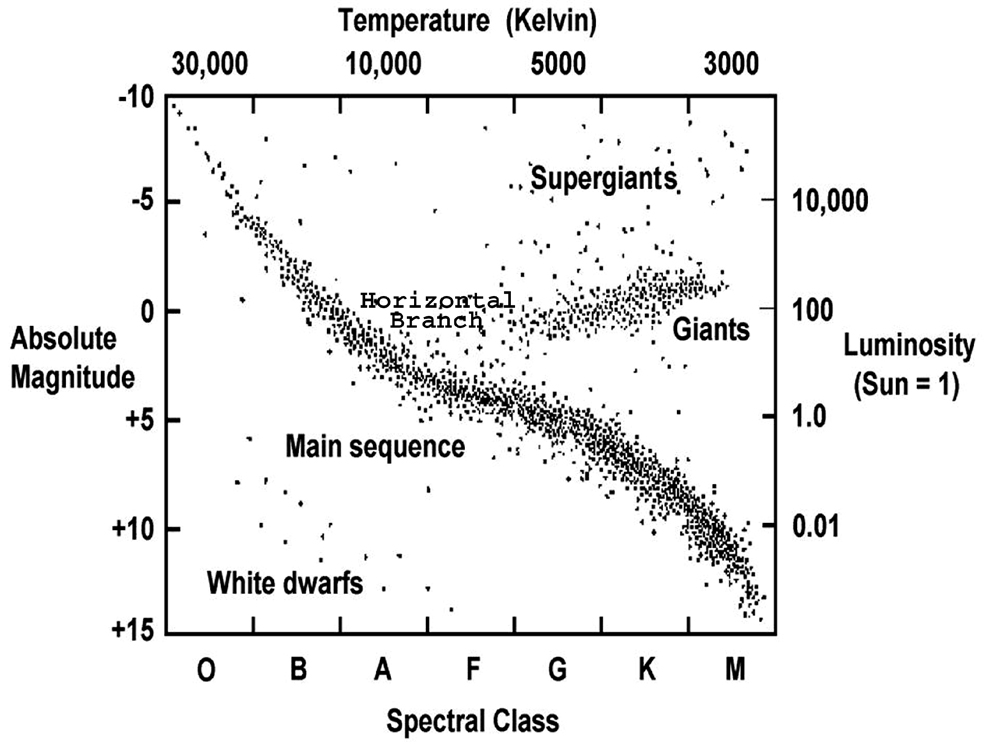
\includegraphics[scale=0.3]{HR_diagram.jpg}
        \\
        Hertzsprung-Russelův diagram\footnotemark
    \end{center}
\end{figure}
\noindent\textbf{Úlohy:}
%<*task>
\begin{enumerate}
\item Proč nevidíme zelené nebo třeba fialové hvězdy?
\item Při pohledu na HR diagram vás možná zaskočilo, že hodnota jednoho dílku stupnice zářivého výkonu (luminosity) neodpovídá hodnotě jednoho dílku stupnice absolutní magnitudy. Co to vypovídá o lidském vnímání zářivosti?
\end{enumerate}
%</task>
\footnotetext{{Ilustrace od Chandra X-ray Observatory edu, NASA}}
\end{document}
